

\subsection{Case Study I: Inertia-Wheel Pendulum}
\label{sec:iwp}

In this section, we apply the design methodology to the problem of stabilizing
the inverted position of an inertia wheel pendulum (IWP), shown in
Fig.~\ref{fig:iwp}. 

This mechanism is a simple pendulum with an actuated wheel instead of a static
bob.
%
The wheel has mass $m$, which is connected to a massless rod of length \(l\). 
%
The rod is connected to ground by a revolute joint, whose position
is denoted by the angle \(\theta_1\) measured with respect to the downward
vertical position.
%
The position of the wheel \(\theta_2\) is measured with respect to the vertical
line through the center of the wheel.

\begin{figure}[tb]
    \centering
    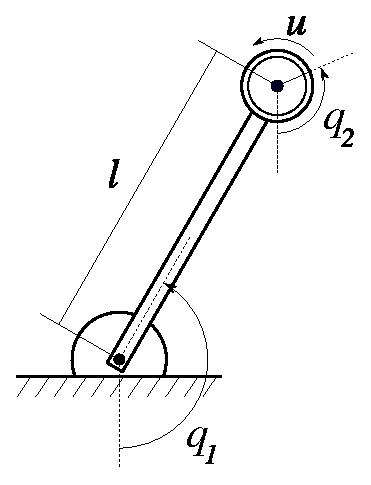
\includegraphics[width=0.27\linewidth]{figures/iwp.eps}
    \caption{Schematic of the inertia wheel pendulum. The rotating wheel \(\theta_2\) is actuated.}
    \label{fig:iwp}
\end{figure}

\subsubsection{System Model}

The Hamiltonian is $H = \frac{1}{2} p^\top M^{-1} p + V(q)$, with $p = \bmat{I_1
\dot{q}_1 & I_2 \dot{q}_2}^\top$ and
%
\begin{equation*}
    M = \bmat{I_1 & 0 \\ 0 & I_2},
    \quad
    G = \bmat{-1 \\ \phantom{-}1},
    \quad
    V(q) = mgl \left( \cos q_1 - 1 \right).
\end{equation*}
%
Here \(I_1\) denotes the moment of inertia of the pendulum, \(I_2\) is the moment of
inertia of the rotating wheel, \(g\) is the gravitational constant, and $l$ is
the length of the rod. The equilibrium to be stabilized is the upward position $(q_1^\star, q_2^\star) = (0, 0)$.
%
The equations of motion of the IWP can be written in standard form as 
%
\begin{equation*}
    % \begin{aligned}
    %     I_1\ddot{\theta}_1 &= -mgl \sin(\theta_1) - u, \\
    %     I_2\ddot{\theta}_2 &= u
    % \end{aligned}
    \bmat{I_1 & 0 \\ 0 & I_2} \bmat{q_1 \\ q_2} + \bmat{-mgl \sin q_1 \\ 0} = \bmat{-1 \\ \phantom{-}1} u, 
\end{equation*}
%
where the control input \(u\) is the torque applied to the inertia wheel.
%
The following values are used for system parameters: \(I_1
= 0.1,\, I_2 = 0.2\), and $mgl = 10$. 


\begin{table}[b]
    \caption{Neural network architectures for solving~\eqref{eq:solve_Md} in the IWP case study. The ordering of the layer dimensions and activations are arranged from input to output. }
    \centering
    \begin{tabular}{r|c|c}
         & Layer Dimensions  & Activation Functions \\ \hline
        $M_d^\theta$ Equation~\eqref{eq:cholesky} & (2, 16, 16, 3) & (ELU, ELU, ELU, Identity) \\
        $U_1^\theta$ Equation~\eqref{eq:skew_symmetric} & (2, 8, 8, 1) & (ELU, ELU, ELU, Identity) \\
        $U_2^\theta$ Equation~\eqref{eq:skew_symmetric} & (2, 8, 8, 1) & (ELU, ELU, ELU, Identity) \\ 
    \end{tabular}
    \label{tab:iwp_nn}
\end{table}

\subsubsection{Controller Design}

We begin by tackling the optimization problem~\eqref{eq:solve_Md} and finding
$M_d^\theta, U_1^\theta, U_2^\theta$. For this particular system, the PDE constraint~\eqref{eq:pde_1}
would have been trivially satisfied if $M_d^\theta$ is a constant matrix, and $U_1^\theta =
U_2^\theta = 0$. However, we demonstrate the flexibility of our approach by having the
learning framework come up with the appropriate solutions (not necessarily the
trivial ones) automatically.

The entries of each of the matrices $M_d^\theta, U_1^\theta, U_2^\theta$ are
outputs of neural networks. The architecture of each network is summarized in
Table~\ref{tab:iwp_nn}. The degree of the SoS polynomial $V_d^\theta$ is 4
($d=2$). In total, there are 1,261 parameters in $\theta$ to train.

To gather the data for training the function approximators, the state space is
sampled uniformly from $q_1, q_2 \in [-\pi, \pi]$, with a step size of $0.1$.
There are a total of 3,969 samples. The collection of these samples are then
shuffled and organized into batches. For each batch, the objective function $J$
of~\eqref{eq:solve_Md} is evaluated, and the gradient descent algorithm updates
the parameters $\theta$ according to its gradient. An iteration is completed
when all samples have been processed. This process is repeated until the
objective value is smaller than a user-defined threshold, or until a maximum
number of iterations is reached.

Fig.~\ref{fig:iwp-projections} shows the progress of the objective value from
the training session. The loss rapidly decreases after only a few iterations.
Each iteration typically takes about 10-15 seconds to perform on an Intel Core
i7-10750H machine without parallel computation. It took 84 iterations to obtain
the results shown in the next subsection. These results demonstrate the data
efficiency of our approach.

% \begin{minipage}{\textwidth}
%     \begin{minipage}[b]{0.45\textwidth}
%       \centering
%       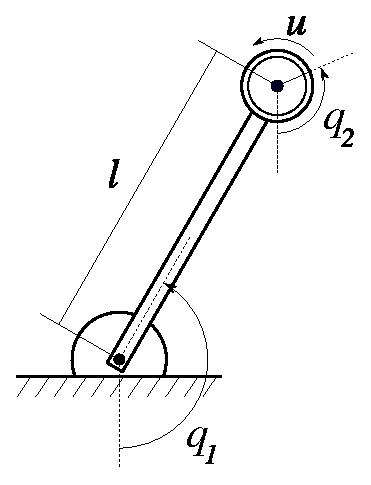
\includegraphics[width=0.5\textwidth]{figures/iwp.eps}
%       \captionof{figure}{Schematic of the inertia wheel pendulum. Only the rotating wheel \(\theta_2\) is actuated.}
%       \label{fig:iwp}
%     \end{minipage}
%     \hfill
%     \begin{minipage}[b]{0.45\textwidth}
%       \centering
%       \begin{tabular}{cc}\hline
%         Table head & Table head \\ \hline
%           Some values & Some values \\
%           Some values & Some values \\
%           Some values & Some values \\
%           Some values & Some values \\
%           Some values & Some values \\
%           Some values & Some values \\ \hline
%         \end{tabular}
%         \captionof{table}{A table beside a figure}
%         \label{tab:iwp_params}
%     \end{minipage}
% \end{minipage}

\subsubsection{Simulations}

We demonstrate the efficacy of our approach through simulation studies. After
training, the swing-up controller is derived according to
Eq.~\eqref{eq:ida-pbc_control},~\eqref{eq:ues} and~\eqref{eq:udi}. The damping
gain $K_v$ in~\eqref{eq:udi} is chosen as the identity matrix.

A simulated trajectory executed using the learned controller is shown in
Fig.~\ref{fig:iwp_evolution}. For this particular simulation, the system starts
at rest with the initial configuration $q(0) = (3,0)$, i.e. the pendulum is near
the downward equilibrium. The controller successfully brings the mechanism to
the desired upright equilibrium.

The results here suggest that approximations to the solutions of the matching
PDEs in the IDA-PBC design methodology is an effective way to algorithmically
find stabilizing controllers for underactuated mechanical systems.

\begin{figure}[tb]
    \centering
    %
    \subfloat[The learned energy-like function $H_d^{\theta}(q,0)$]{%
    \resizebox*{0.45\linewidth}{!}{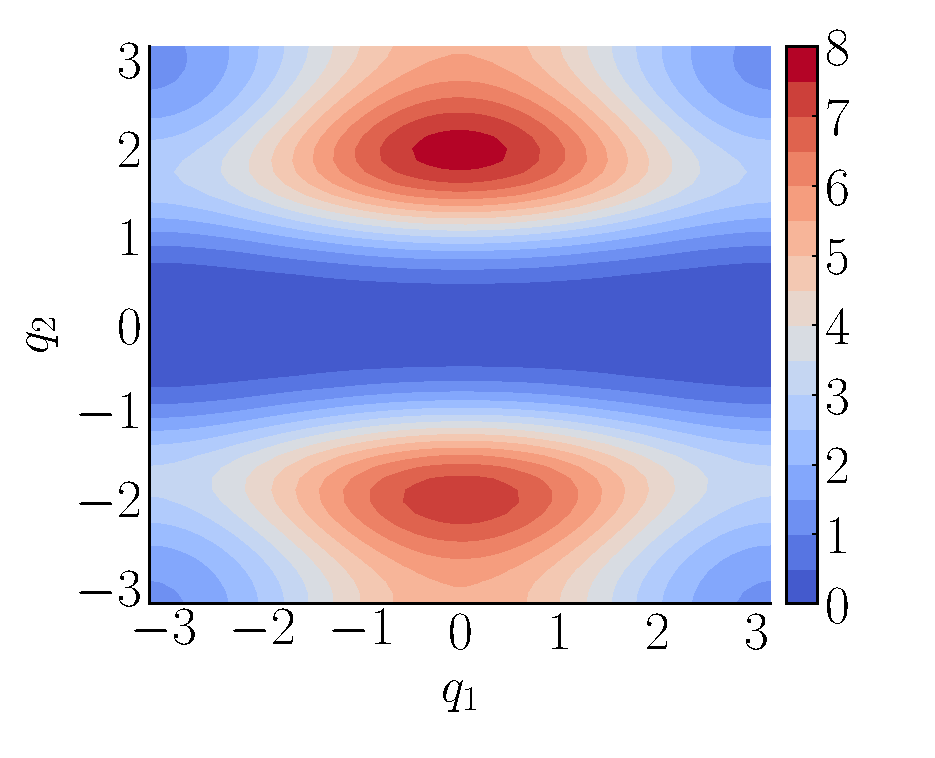
\includegraphics{./figures/contour_Hd_02.eps}}}
    % \label{fig:iwp-projections}
    %
    \hspace{5pt}
    %
    \subfloat[The objective value of Eq.~\eqref{eq:solve_Md} during training]{%
    \resizebox*{0.46\linewidth}{!}{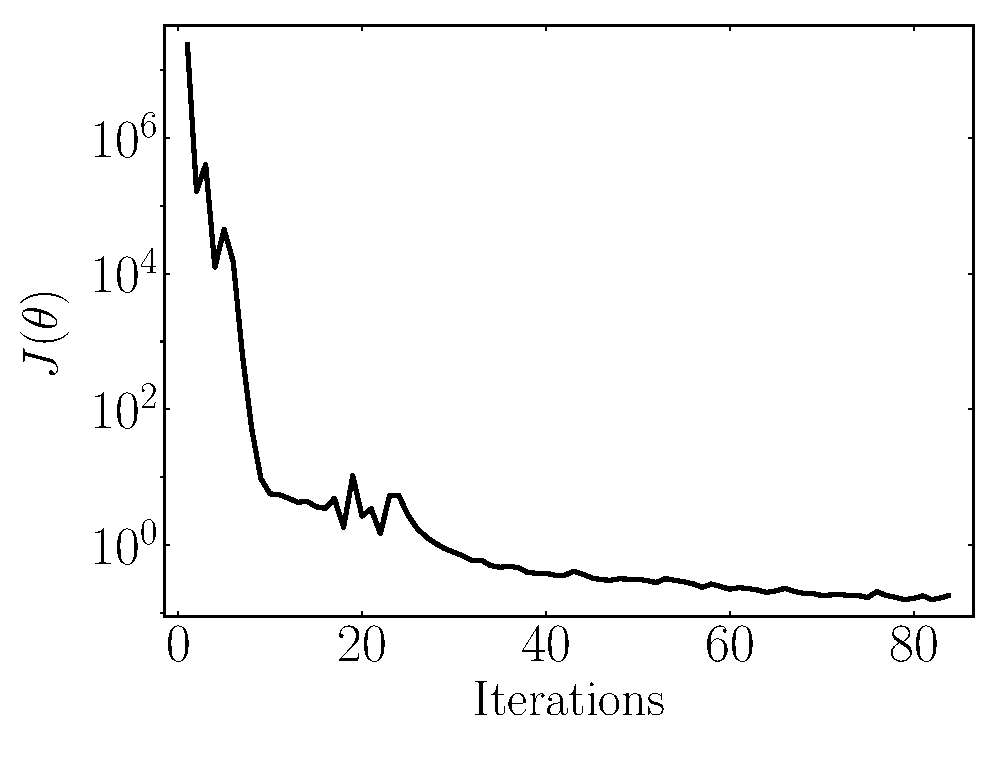
\includegraphics{./figures/loss.eps}}}
    % \label{fig:iwp-loss}
    %
    \caption{(a) Projection of the energy-like function $H_d^\theta$ after training and (b)
    the loss of the PDE constraints~\ref{eq:pde_1} rapidly decreasing during training.}
    %
    \label{fig:iwp-projections}
\end{figure}

\begin{figure}[tb]
    \centering
    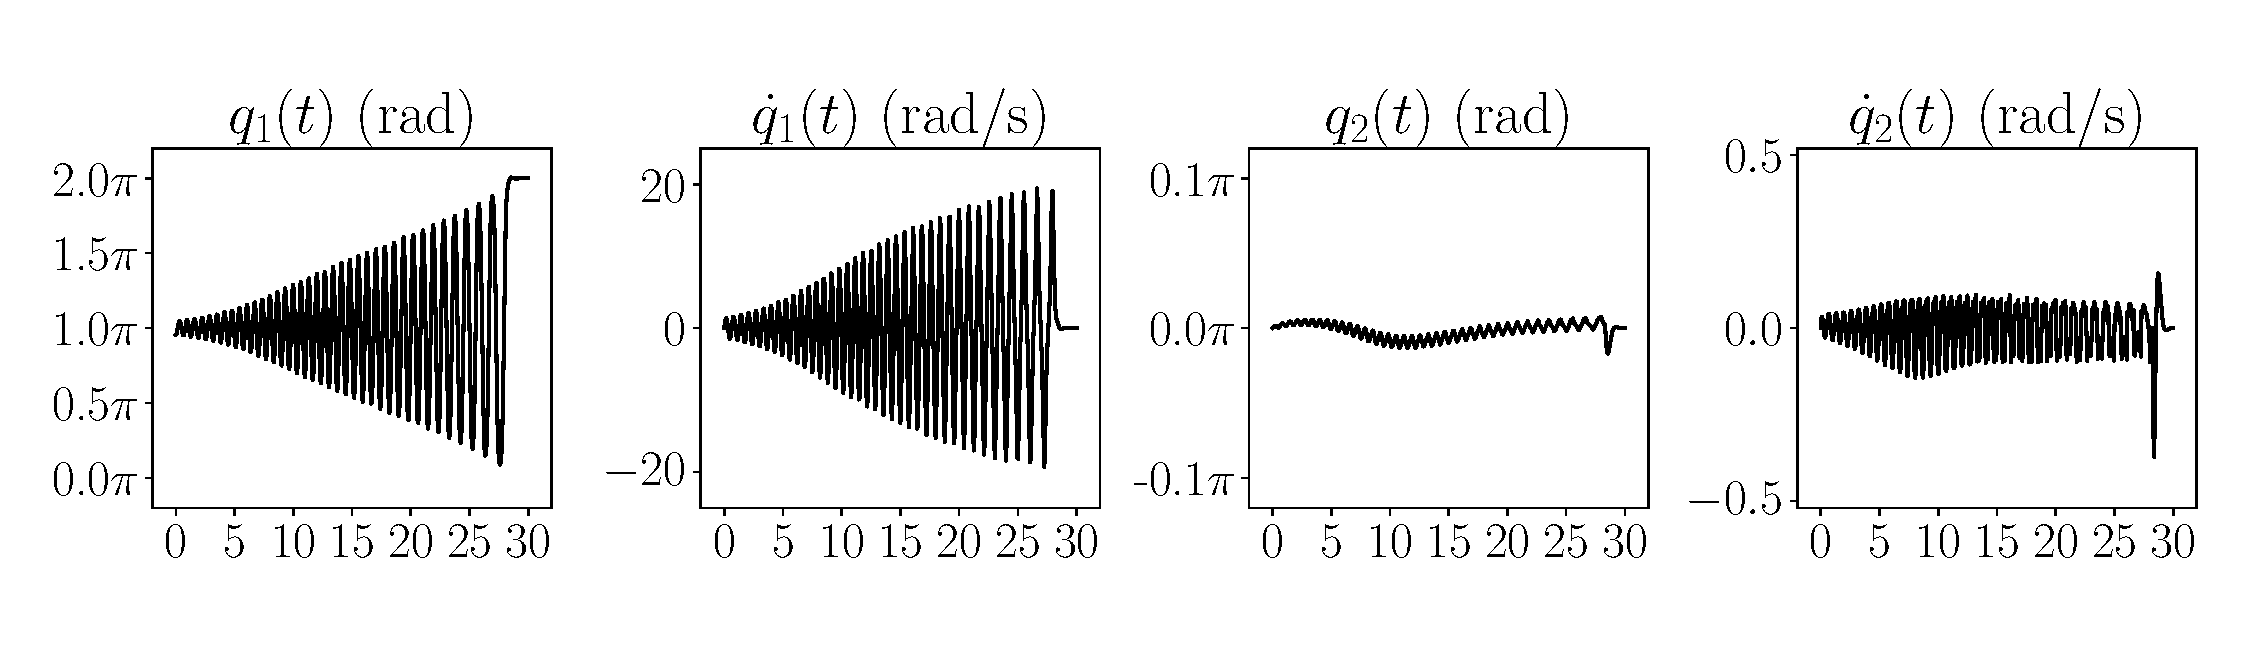
\includegraphics[width=\linewidth]{iwp_evolution.eps}
    \caption{Time evolution of inertia wheel pendulum with the data-driven IDA-PBC.}
    \label{fig:iwp_evolution}
\end{figure}